\documentclass[12pt]{article}
\usepackage[margin=1.2in]{geometry}
\usepackage{color}
\usepackage{graphicx}
\usepackage{url}
\usepackage{amsmath}
\usepackage{amssymb}
\usepackage[round]{natbib}
\bibliographystyle{evolution}
\usepackage[usenames,dvipsnames,svgnames,table]{xcolor}


%\bibliographystyle{abbrvnat}
%\setcitestyle{authoryear,open={(},close={)}}
\usepackage[innercaption]{sidecap} % side captions
\sidecaptionvpos{figure}{c}

\begin{document}

\title{Project Narrative: The genetic archaeology of modern maize breeding: identifying useful diversity through historical pedigree reconstruction}
\author{}
\date{}
\maketitle

\section*{Rationale and Significance}
\label{sec:rationale}

Maize is a natural resource of fundamental national importance, vital for food, livestock feed, and fuel production.
Maize is also the most valuable field crop in the United States, with production values at greater than \$50 billion dollars every year since 2010 \citep{usdanass}. 

But while maize yields have increased over the last several decades, the rate of gain falls short of projected needs in the near future.
% * <jholland@ncsu.edu> 2015-03-30T18:46:15.836Z:
%
%  http://www.nature.com/ncomms/2013/131217/ncomms3918/full/  This paper shows essentially a linear trend in corn yield gains in the past 40 years, but argues that the R&D investment has increased faster than the rate of gain, suggesting increase per investment is decreasing. (most field breeders would blame that on investment in molecular research, but investments in scale of field testing in private sector have been increasing as well. This is a debated area, but I think your main point is basically correct.)
%
Even under stable climatic conditions, current rates of maize improvement are insufficient to meet requirements of population growth over the next 30 years \citep{ray2013yield}; in  addition to requirements in terms of food and animal feed, worldwide ethanol use is projected to increase 40\% within just the next decade \citep{usdalong}.
%could be convinced to drop the ethanol comment

Changing climatic conditions, however, will likely further challenge our ability to meet needed yield gains. 
Historical analyses suggests that climate change over the last 30 years has already dramatically impacted maize yields worldwide, retarding gains from breeding and management \citep{Lobell2011}.
Moreover, predicted temperature increases will increase volatility in yield across the U.S. and may even decrease future yields \citep{urban2012projected}, with some models suggesting a change of even 1$^{\circ}$C could negatively impact yields by as much as 17\% \citep{lobell2003climate}; more dire warnings suggest that U.S. maize yields could drop 30-46\% below current levels by the end of the century \citep{schlenker2009nonlinear}.
Substantial efforts will clearly be needed to preserve U.S. maize production and increase or maintain yields.  

Much of the historical gains in maize yield can be directly attributed to breeding efforts \citep{Duvick1992, duvick2005genetic}, and {\bf breeding must remain of central importance in order to meet increased yield demands}.  
Breeding is also of key importance in adapting maize to the challenges of changing climates \citep{Troyer2004a}, with recent models suggesting that efficient use of extant adaptive diversity in maize could significantly ameliorate the effects of climate change \citep{butler2013adaptation}.   

\subsection*{Diversity loss threatens breeding gains}

Breeding, and adaptation in general, relies critically on the availability of genetic diversity. 
This is best represented mathematically by JL Lush's famous ``breeder's equation'' $R=\frac{V_a}{V_p}s$, showing that adaptation --- the response to selection $R$ --- depends not only on the strength of selection $s$ but also directly on the amount of heritable genetic variation $V_a$ for the trait of interest \citep{kelly2011breeder}. 
The advent of modern hybrid maize breeding, the development of distinct breeding pools and the winnowing of inbreds from individual breeding programs has led to a marked decrease in genetic diversity (Figure 1). 
Analyzing genotypes of more than 4000 public and recently released private lines, we recently showed that the diversity available to maize breeders in current germplasm is less than half what it was in before 1950 (Figure \ref{fig:diversity}). 
With decreasing diversity available for breeding decreasing yield gains are a mathematical certainty. 
%over the top?

\begin{SCfigure}[][t]
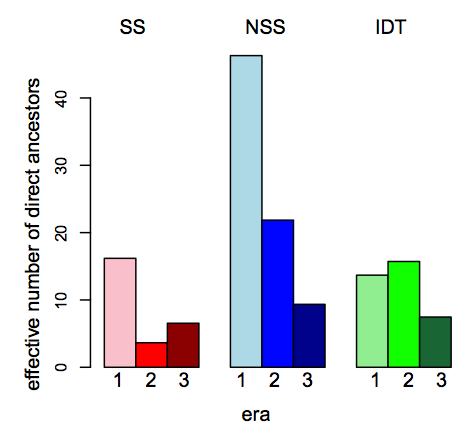
\includegraphics[width=0.5\linewidth]{joost_diversity.png}
\caption{Changes in genetic diversity (represented as the effective number of ancestors) of the three primary maize heterotic groups (SS: stiff-stalk; NSS: non-stiff-stalk; IDT: iodent). Inbreds are divided into eras representing different time periods: 1:1930-1950; 2:1950-1980; 3:1985-1992. Figure from \citet{van2012historical}.} 
\label{diversity}
\end{SCfigure}

While open-pollinated varieties and exotic inbred lines represent a viable source of new diversity, these have been only sparingly used in the private sector due to their poor agronomic performance, photoperiod sensitivity, and the necessary generations of back-crossing to adapted lines required to incorporate useful alleles into high-performing temperate germplasm \citep{goodman1999broadening}.
In contrast, older U.S. inbred lines, though lower-yielding than their contemporaries, harbor novel genetic diversity of potential use for breeding but are already adapted to the U.S. cornbelt.  
For example, a recent phenotypic evaluation identified several older inbreds as sources of useful variation for drought and heat tolerance \citep{chen2012characterization} and our own population genetic analysis identified a number of older inbreds enriched for underutilized adaptive alleles (Figure \ref{fig:wf9}).
%http://www.jswconline.org/content/67/5/354.full.pdf
% identified B76 -- iowa line from 1974 that did not contribute as much to current pedigrees, vs B73 which is more important pedigree-wise
%COME BACK TO THIS POINT IN INTRO -- BOTH SHOW FAVORABLE ALLELES NOT ALWAYS USED IN MODERN

\begin{SCfigure}
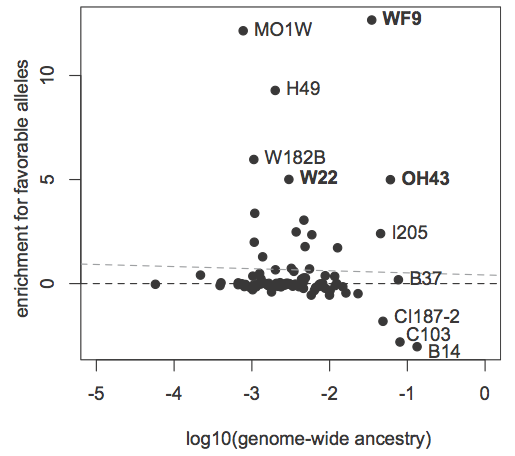
\includegraphics[width=0.5\linewidth]{joost_wf9.png}
\caption{Enrichment (defined as the log probability ratio with respect to control loci) of favorable alleles in older (era 1) inbreds as a function of their average ancestral contribution to modern (era 3) lines. The black dotted line represents the 0 horizontal, and the gray dotted line the regression  with slope −0.1). Inbred names are shown for lines with log probability ratios higher than 4 or ancestry proportion above 0.03. Labels in boldface mark breeding lines of known historic popularity. Figure from \citet{van2012historical}.} 
\label{fig:wf9}
\end{SCfigure}

\subsection*{Lack of public resources limits use of diverse germplasm}

Breeders will not blindly incorporate older material into their populations, however.  
Perhaps the most important piece of information required to effectively utilize older germplasm is pedigree.
Pedigree data immediately gives a breeder information on crosses likely to produce higher yields due to heterosis, and often provides additional utility in identifying likely maturity (flowering time) and other agronomic characteristics. 
Combined with phenotype data, pedigree information can even be used to predict phenotype even in the absence of genotype \textcolor{red}{CITE} and pedigree-based methods for identifying useful diversity have already been patented by industry \citep{sebastian1995method}.
% * <jholland@ncsu.edu> 2015-03-30T18:55:39.680Z:
%
%  actually, given pedigree data ALONE, you can predict breeding values if  you have some relatives measured for traits. see Bernardo's BLUP papers of mid 90s
%

While private industry may in many cases have detailed records of their own breeding material, the vast majority of private germplasm is founded on $20^{th}$ century public breeding lines \textcolor{red}{CITE}.
% * <jholland@ncsu.edu> 2015-03-30T18:56:49.240Z:
%
%  discussed to some extent in Nelson et al 2008 ex pvp paper
%

Unfortunately, pedigree data for most U.S. maize inbreds is unavailable to most breeders. 
For example, of the \textcolor{red}{XXX} inbreds in the USDA Germplasm Resources Information Network, only \textcolor{red}{XXX}\% have both parents identified. 
While there are published compilations of germplasm, these are far from complete:  \citet{gerdes1993compilation}, for example, contains complete pedigree data for less than \textcolor{red}{XXX}\% of the germplasm in the USDA database.
Moreover, what ancestry information that is available is not in electronic form nor easily accessible in any single resource.  
Instead, historical pedigree information exists primarily in the minutes of breeding committees, old breeding program books, and other hard-copy sources with limited distribution.  

{\bf We propose to  generate an open-source database of public maize pedigrees and genotypes and use this resource to identify genotypic and phenotypic diversity of high utility in advancing maize breeding.}
%this reads too long, efforts to shorten are welcome.
Given the importance of maize to U.S. agriculture, this proposal clearly aligns with the USDA AFRI program priorities of ``Plant Breeding for Agricultural Production.''  
Our proposal will develop tools to accelerate breeding by allowing breeders to more quickly identify useful inbreds, and our application of population and quantitative genetic methods will identify specific genetic and phenotypic diversity of potential use for future breeding.  
%do we say something about ``Development and application of tools to predict phenotype from genotype to accelerate breeding of finished varieties;'' (from the RFA)??

\section*{INTRODUCTION}
\label{sec:introduction}

%a. Introduction
%Include a clear statement of the long-term goal(s) and supporting objectives of the proposed project. Summarize the body of knowledge or past activities that substantiate the need for the proposed project. Describe ongoing or recently completed activities significant to the proposed project including the work of key project personnel.

\begin{itemize}
\item history of maize breeding
\item show decline of yield
\item show loss of diversity
%joost, gerke
\item diversity needed for selection to function, breeder's equation
\item weaknesses with previous approaches
\item pedigree data allows idnetificaiton of direct action of breeder selection
%citep some lit on allele dropping!!
\item Preliminary work: Howie's inbred pedigrees
\item Preliminary work: Kate pedigree building
\item preliminary work: GBS pruning pedigree
\item preliminary work: allele dropping works?
\end{itemize}

\subsection*{Maize breeding}
Maize has undergone dramatic phenotypic and genetic changes since its domestication and subsequent spread through North and South America \citep{daFonseca:2015ey,Doebley:2004ce}. More recently, beginning in the mid-20$^{th}$ century, the intensification of maize breeding efforts has lead to subtler but equally important changes including increasing yields and improved agronomic traits such as leaf angle and density tolerance \textcolor{red}{CITE}. 

%, but also significantly impacting patterns of genetic diversity \citep{Duvick:2001fy,van2012historical}.

Maize is  a self-compatible crop, and modern breeding programs (post-1960) take advantage of self-fertilization (or now double-haploid technology) to create homozygous inbred lines. 
Distinct inbreds are maintained in separate breeding pools or heterotic groups.
The most important heterotic groups among U.S. public germplasm are the ``stiff stalk'', ``non-stiff stalk'', and ``iodent'' (Figure \ref{fig:diversity}).
Inbred lines from separate breeding pools are then crossed to make hybrid progeny.  
These hybrids often display heterosis, meaning that yield and associated traits of the hybrid are superior to  either inbred parent \citep{Springer:2007bj}.  
Inbreds capable of producing high-yielding, heterotic offspring are said to have good ``combining ability'', and are recycled in their respective breeding pools.
Inbreds that form less desirable combinations are usually discarded from the breeding pool. 
Useful inbreds within a group are crossed with each other, and their segregating progeny evaluated and self-fertilized to create new inbreds. 
Maintaining this system for propagation of inbred lines and hybridizing inbreds for evaluating production traits has worked well for many decades, but there is growing reason for concern that this method may need a genetic boost. 

\subsection*{Decreasing diversity} 

Our analysis of the Iowa Reciprocal Recurrent Selection program provides an insight into how modern breeding programs impact genetic diversity. 

A set of founding genotypes 

\begin{figure}
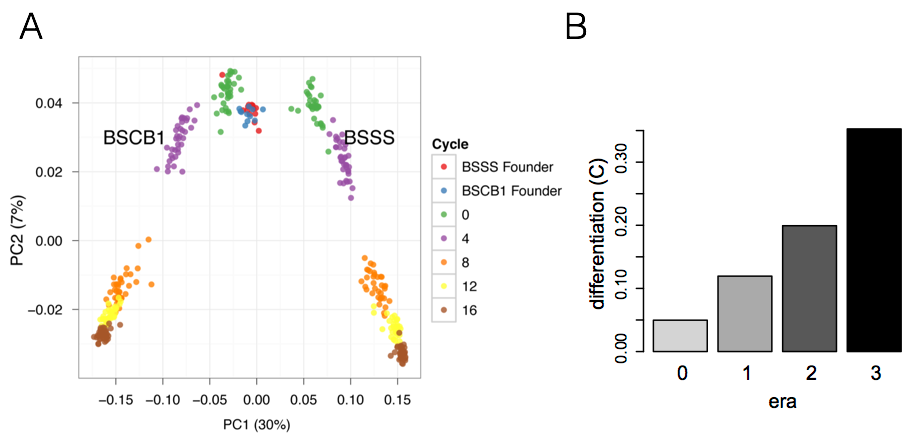
\includegraphics[width=\linewidth]{joostgerke}
\caption{Changes in diversity and population structure during maize breeding.  
A) Principal component analysis of genotypes from the Iowa Reciprocal Recurrent Selection population. The first eignevector represents divergence between the two heterotic pools, and the second divergence over time within each pool. Figure from \citet{Gerke:2013tw}. 
B) Population structure --- quantified by the differentiation statistic C --- over time across all U.S. public inbreds. Eras represent time periods in Fig. \ref{fig:diversity}; figure is from \citep{van2012historical} } 
\label{fig:pca}
\end{figure}

Maize yields have increased since the 1930s when breeders and farmers first began to adopt hybrid maize.
\textcolor{red]{JRI HERE}
The pace at which yield gains are made, however, has slowed: since the late 1960's the rate of gain of yield has slowed, while maize yields continue to increase, the velocity at which they are increasing has slowed in the modern era (since the 1970s) (Figure \ref{fig:piecewise}). 
% * <jholland@ncsu.edu> 2015-03-30T19:00:00.051Z:
%
%  see Cassman paper mentioned above, the trend appears linear. the issue may be gain per investment effort.
%
 (Figure: \ref{fig:piecewise}).
While some of this improvement has resulted from changing management practices, it is probable that much of the change in yield over time is due to the success of breeding programs in producing hybrids capable of producing high yields under stress and in combination with modern agronomic practices.  \citep{Duvick:2001fy}. 

Removing the effect of input of nitrogen and other fertilizers from yield each year reveals that a good portion of the variation in yield is due to genetics (and possibly other environmental factors) (Figure\ref{fig:inflection}. 
We propose here that the major cause that is contributing to this observed slowing yield may be the drop in genetic diversity. 
It has been shown that while diversity has increased amongst inbred lines \citep{Gerke:2013tw}; the within population level haplotype diversity of modern inbred lines \citep{van2012historical} has dropped over time. 
% * <jholland@ncsu.edu> 2015-03-30T19:05:15.855Z:
%
%  is this the BSSS paper? can its results be inferred to all of USA maize? this might need clarification.
%
Maize inbreds from different breeding pools are rarely (if ever) crossed for propagation, and beneficial/adaptive alleles are only meeting during hybrid test crosses. 

This drop within separate inbred line breeding pools is likely due to the current breeding practice of discarding inbred lines out of the breeding population or pool if they do not show favorable combining ability (thus, alleles are gradually discarded within a population).  
We contend that this genetic diversity within a breeding pool or population needs to be recovered in some way.  
% * <jholland@ncsu.edu> 2015-03-30T19:07:13.871Z:
%
%  the reaction by breeders to this is likely to be: such lines are dropped for good reason, and breeding gains may require some loss of diversity, since much of diversity is not favorable. i wonder if the objective needs to be something more like identifying this lost diversity is important assuming that SOME of those alleles are useful and were lost due to drift, negative hitchiking, or whatever. I bet there are many of those alleles that no breeder wants to see again, inbred performance is just so much better now than 50 years ago.
%

Perhaps of greatest concern for the future of maize breeding, is that much of the original diversity from inbreds used to create modern hybrids used jointly by public researchers and industry has dropped over time \citep{Gerke:2013tw}. 
This inherently means a reduced response to natural and/or artificial selection, and indicates that there will be only diminishing returns on yields as time goes on unless new diversity is brought back into breeding pools. 
Recombination between current commercial inbred lines creates only new genotypic combinations of alleles, not new diversity and new mutational inputs over the short term that are not neutral are likely to be deleterious.

\begin{figure}[ht]
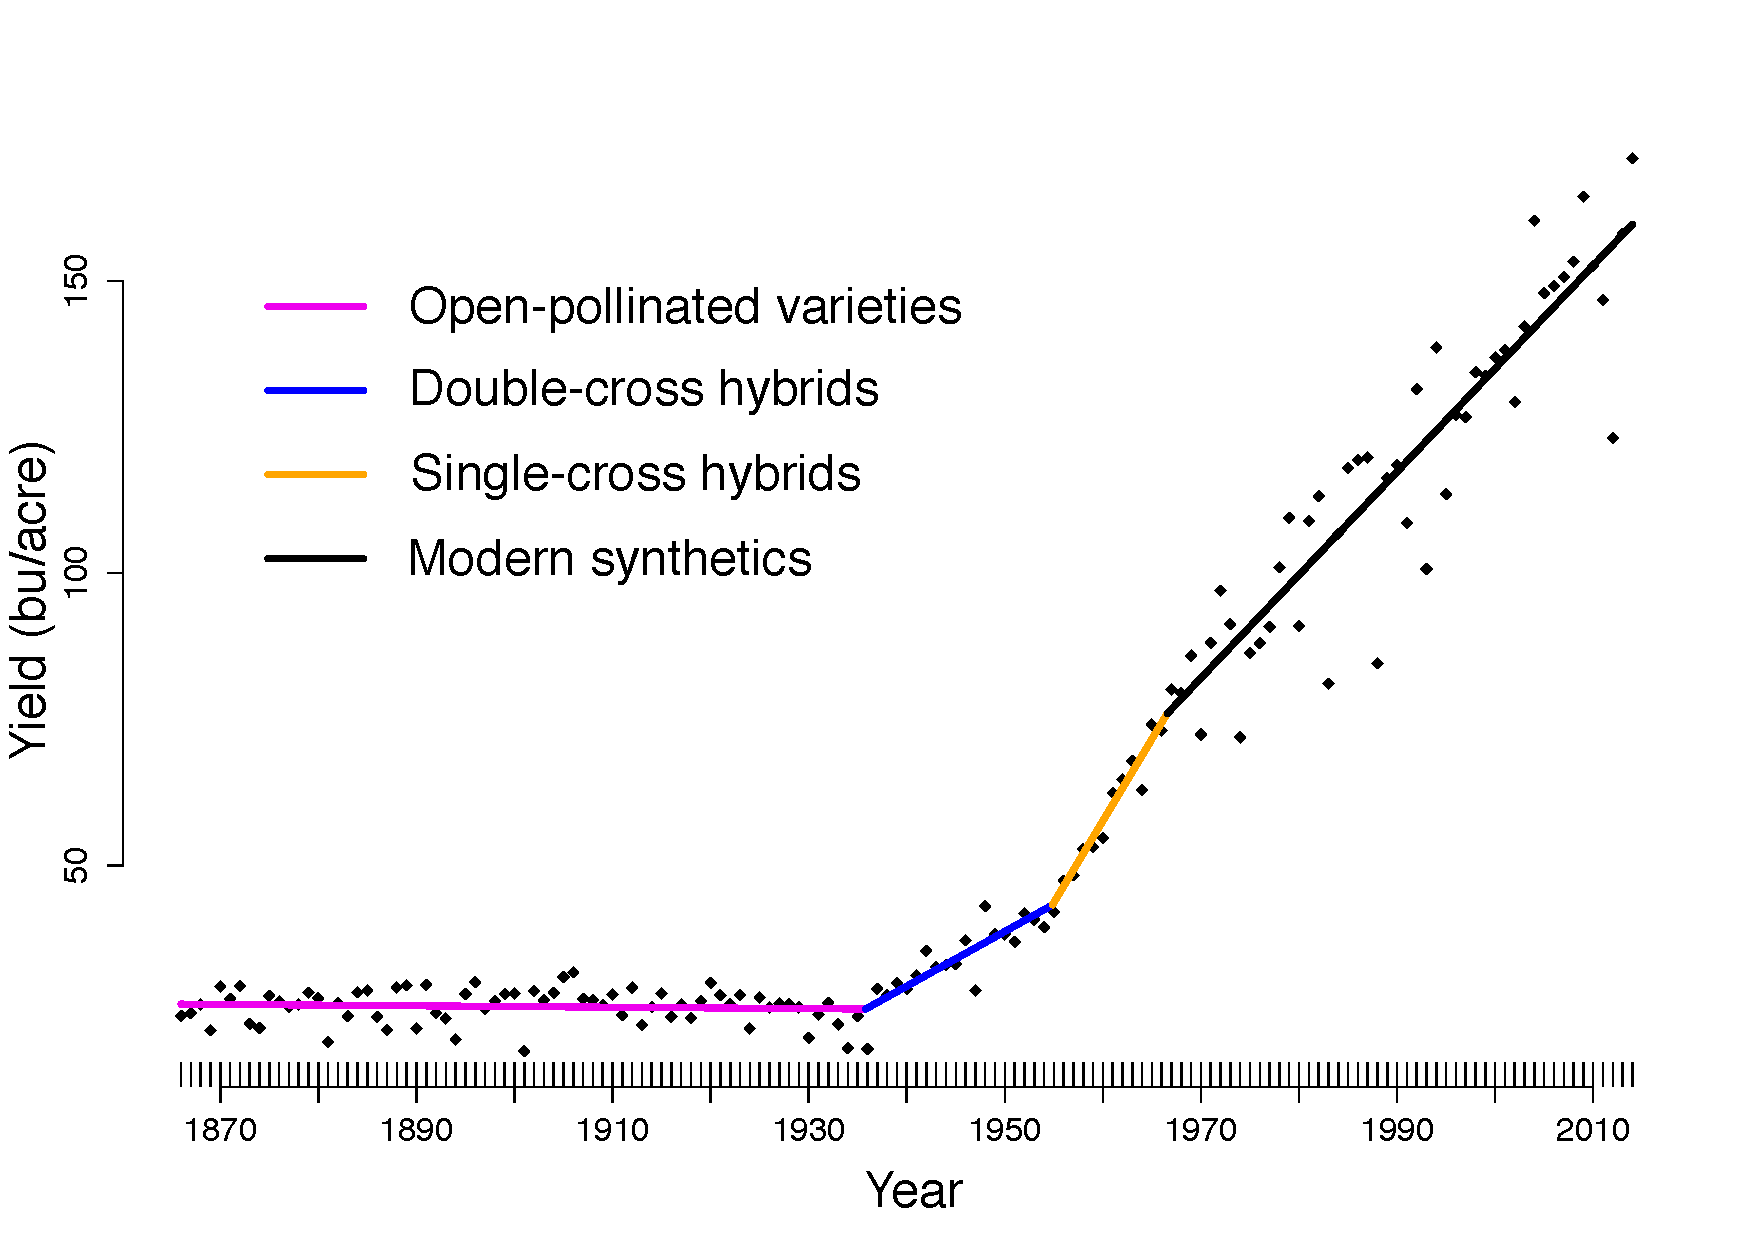
\includegraphics[width=1.0\linewidth]{yield.pdf}
\caption{Piecewise regressions of time against total yield through the four eras of modern maize breeding. Lines correspond to distinct eras of maize breeding.} 
\label{fig:piecewise}
\end{figure}

\begin{figure}[ht]
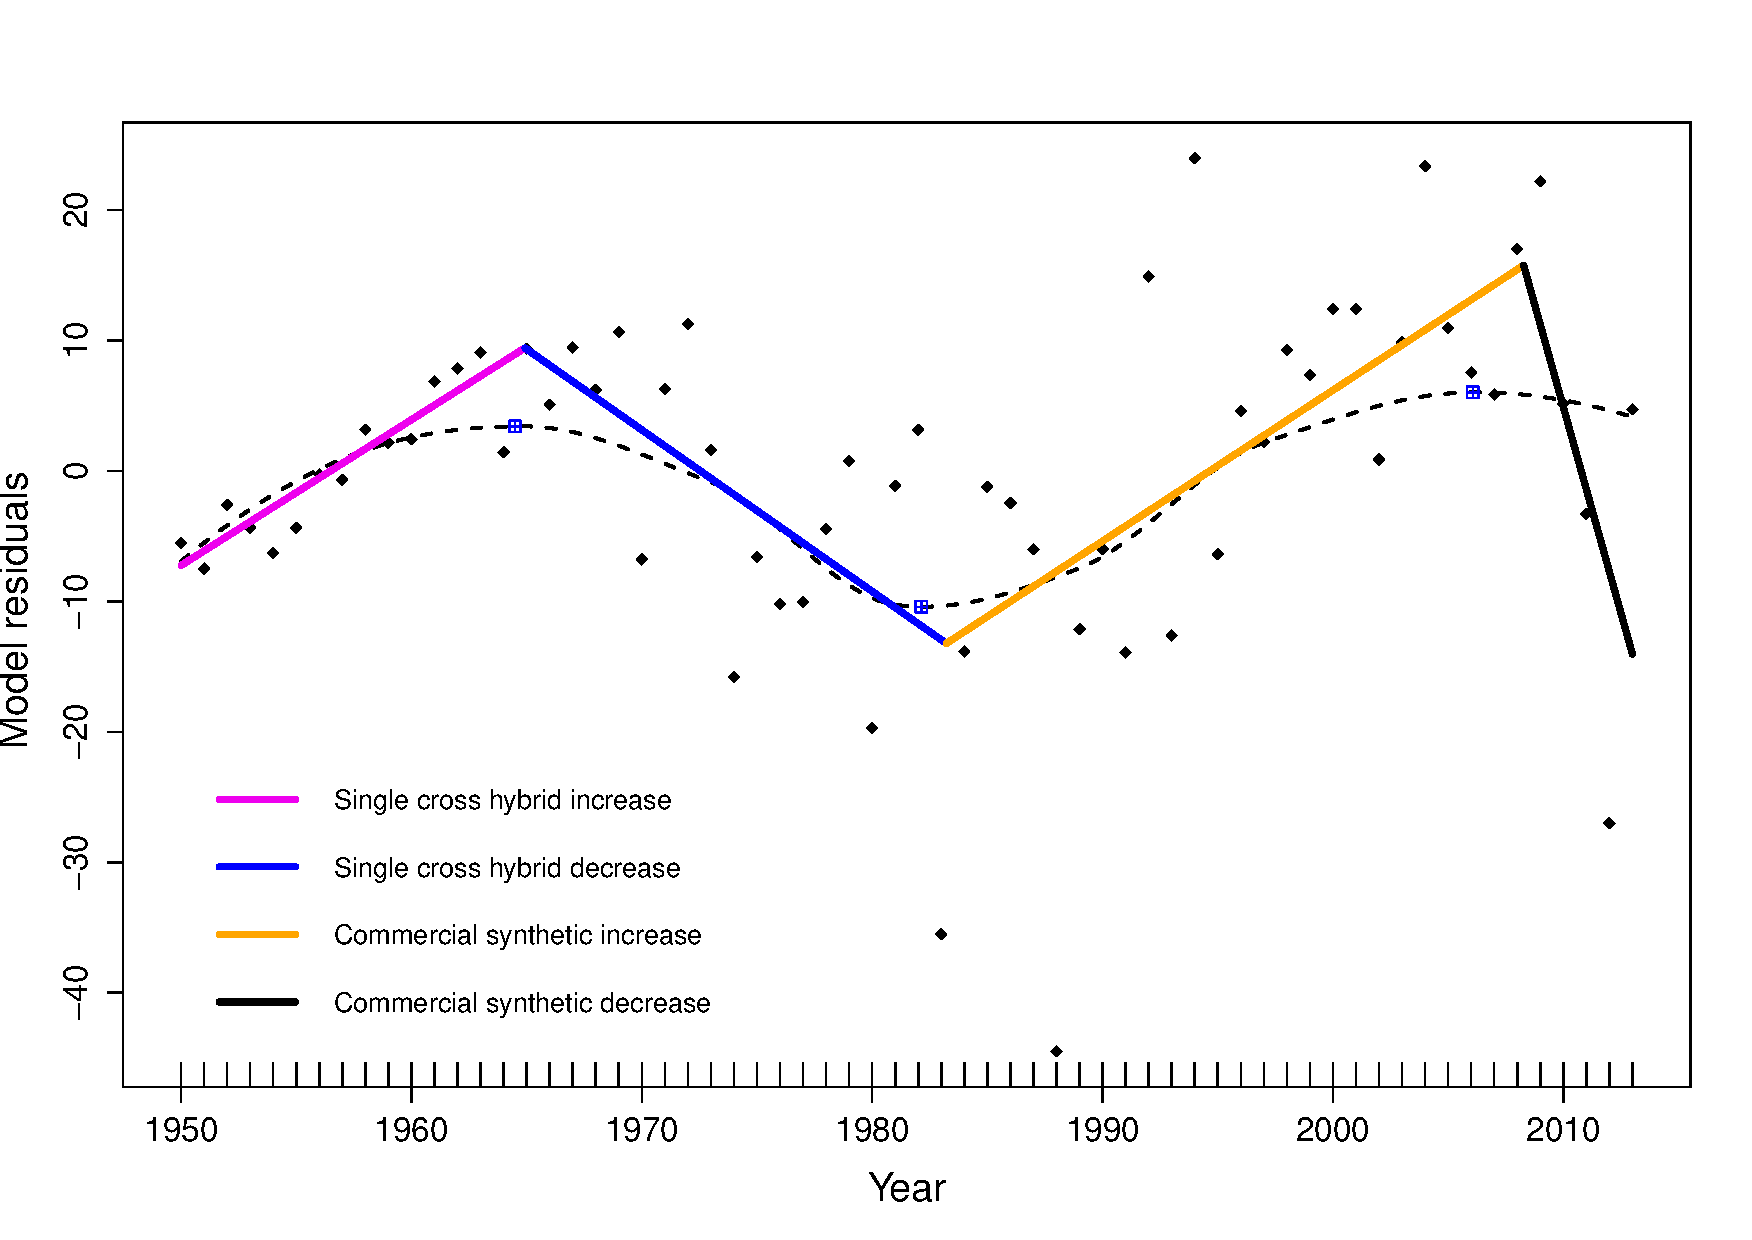
\includegraphics[width=1.0\linewidth]{inflection_point.pdf}
\caption{Model residuals after removing the effect of nitrogen from Figure \ref{fig:piecewise}, with inlection points (blue squares) and piecewise regressions showing the possible points allelic gains and losses through time.} 
\label{fig:inflection}
\end{figure}

\subsection*{Future diversity - ghosts of maize past: A novel approach to incorporate new diversity}

Incorporating novel diversity into contemporary modern maize lines can occur in two ways, by introgressing modern lines with open pollinated landraces from the tropics not previously incorporated into any breeding program. Or, alternatively, 
% * <jholland@ncsu.edu> 2015-03-30T19:13:28.362Z:
%
%  ??
%
. Pedigrees when combined with modern genomic and phenotypic trait data are useful tools not only for tracking loss in allelic diversity, but for identifying loci that have experienced strong artificial selection across breeding pools. Examples of their application can be found with: cattle \citep{Decker:2012kd}, soybean (cite), and grape (cite). 
While private companies likely have their own pedigree databases to do exactly this, these data are private, patented, and not available to the public. 
Further, much of the pedigree information on older founder inbred maize lines sits in old volumes of crop science, release sheets, or breeding books, unused and vulnerable to loss.
% * <jholland@ncsu.edu> 2015-03-30T19:12:23.592Z:
%
%  might want to say Agronomy Journal, since it goes back much longer than Crop Sci (which started in '60). Also experiment station technical bulletins and regional corn breeding meeting records.
%
\subsubsection*{Missing or incomplete data}
\par The National Plant Germplasm Service database contains information with regards to ancestry of public maize inbred lines, much of this information is incomplete or missing. Or it does not 

\textbf{However, much of this ancestry information on modern maize lines  is still publicly available, only not in digital form, nor is it easily-accessible. This historical pedigree information exists in old volumes and minutes of breeding committees, old breeding program books, and other hard-copy-only sources. Here, we propose a project that will help preserve, maintain, and use this historical information with novel genomic data to better benefit future maize breeding programs.} 

\section*{APPROACH}
\label{S:3}
Our proposed research has three major aims in using pedigree information to detect change in diversity of modern inbred maize lines.

% “Small-scale evaluation of individual lines.” These are the grow-outs of individual awesome old lines. need some methodology here — we can’t do crosses, but we can collect good phenotype data on lines. so i would propose:

%year 2) 100 lines of interest in the pedigree, either because of how few or how many offspring they have.  especially focus on those without genotype data.  grow up and get phenotype and genotype
%year 3) 100 lines of known genotype (50 good genotypes 50 bad). grow these up to both i) test phenotype prediction from Qx and ii) see whether lines with lots of good alleles are agronomically superior to lines without

%explain we don’t have the time or resources to actively test these in hybrid yield trials, but this gets preliminary information breeders and industry could use to make decisions about including some of these lines and allows us some ground-truthing of the methods.  we should grow a set of say 20 exPVP lines in each year to compare across years and use as a standard

\begin{itemize}
\item Aim 1: Digitize and curate pedigree and genotype information into a publicly available database. 
\item Aim 2: Identify adaptive alleles using a combination of pedigree and population genetic approaches.
\item Aim 3: Phenotypic and genotypic evaluation of small numbers of individuals lines that feature heavily in the historical pedigree.

\end{itemize}
\subsection*{Proposed activities, methods \& feasibility}
\subsubsection*{Travel and digitization of records and agreed upon database format for all data}
The first part of our proposal aims to preserve hard-copy pedigree records by traveling to different land grant institutions by digitizing them. These raw data scans will then be manually translated into an agreed upon format, with numbering/naming of each line/accession agreed upon.
Dr. Kate Crosby, Dr. Taner Sen (support letter from maize GDB enclosed), senior personnel Dr. Oscar Smith, and CO-PI Dr. Bill Tracy will consult on an agreed upon standard format with which to store the raw scan of pedigree records, the phenotypic and genomic information. Establishing an agreed upon format in the first few months of the project will enable easy mapping of current and future genomic data formats to pedigree information.
\par Additionally, Dr. Kate Crosby is currently investigating the possibility of using no-SQL database without formal schemas specified \textit{a priori} (graph databases) to be able handle queries with respect to mapped genomic data, extended ancestry, and phenotypic data, along with new visualization tools \citep{ParejaTobes:2015bf}.



\subsubsection*{Genotyping of lines that feature heavily in historical pedigree information}
Undoubtedly, there will be information garnered from historical pedigree information on lines that do not have any genomic data available for them. In such cases (where germplasm is available), we intend to use genotype-by-sequencing (GBS) \citep{Elshire:2011ha} as a cost-efficient platform \citep{Glaubitz:2014eu} to obtain genomic data for such lines, with markers aligned to the newest maize reference genome (currently B73 v. 3). 

\subsubsection*{Project 1 for student 1: understanding the dynamics of selection through time with allele-dropping and pedigree}
In the section above we mention that certain maize lines feature heavily in the historic pedigree. For example, in the public pedigree B73 features heavily as a parent to many ancestors of current inbred lines (Figure \ref{fig:b73isbig}). 


\begin{figure}[ht]

\includegraphics[width=1.0\linewidth]{pedigree_poster.pdf}
\caption{Example of a modern maize inbred line that features heavily in the overall pedigree, B73, with numerous inbred progeny.}
\label{fig:b73isbig}
\end{figure}

\par The first masters student to be supervised by Dr. James Holland (NC State) will, with the cooperation of Dr. William Tracy, Dr. Sherry Flint-Garcia, Dr. Oscar Smith, and the post-doc Dr. Kate Crosby use the information gathered during the first year to identify these historically important lines. Many small pedigrees will be constructed from lines identified as having many inbred ``progeny''. This student will then identify distorted segregation at all heterozygous loci (using GBS markers) within and across these many small pedigrees (Figure \ref{fig:alleledrop}), this is known as \textbf{``allele-dropping''}. It is a simple Mendelian approach to identifying traces of selection by directly accounting for ancestry, and without the worry of having to account for shared population structure (as in modern population genomics approaches). If we can identify the uni-directional shift of a given allele across many of these small pedigrees at a set locus, this would indicate selection. 
\par The student would also be responsible for simulating allele frequency change under neutral processes (genetic drift). The approach would be similar to that used in \citep{Gerke:2013tw}, to evaluate at which loci adaptive (by breeders) or neutral forces have shaped the current allelic diversity of the overall modern breeding population. 
\par Should loci be identified as having uni-directionally shifted through time across many of these small pedigrees, we would compare this to our findings in project 2 (see next section).

\begin{figure}[p]
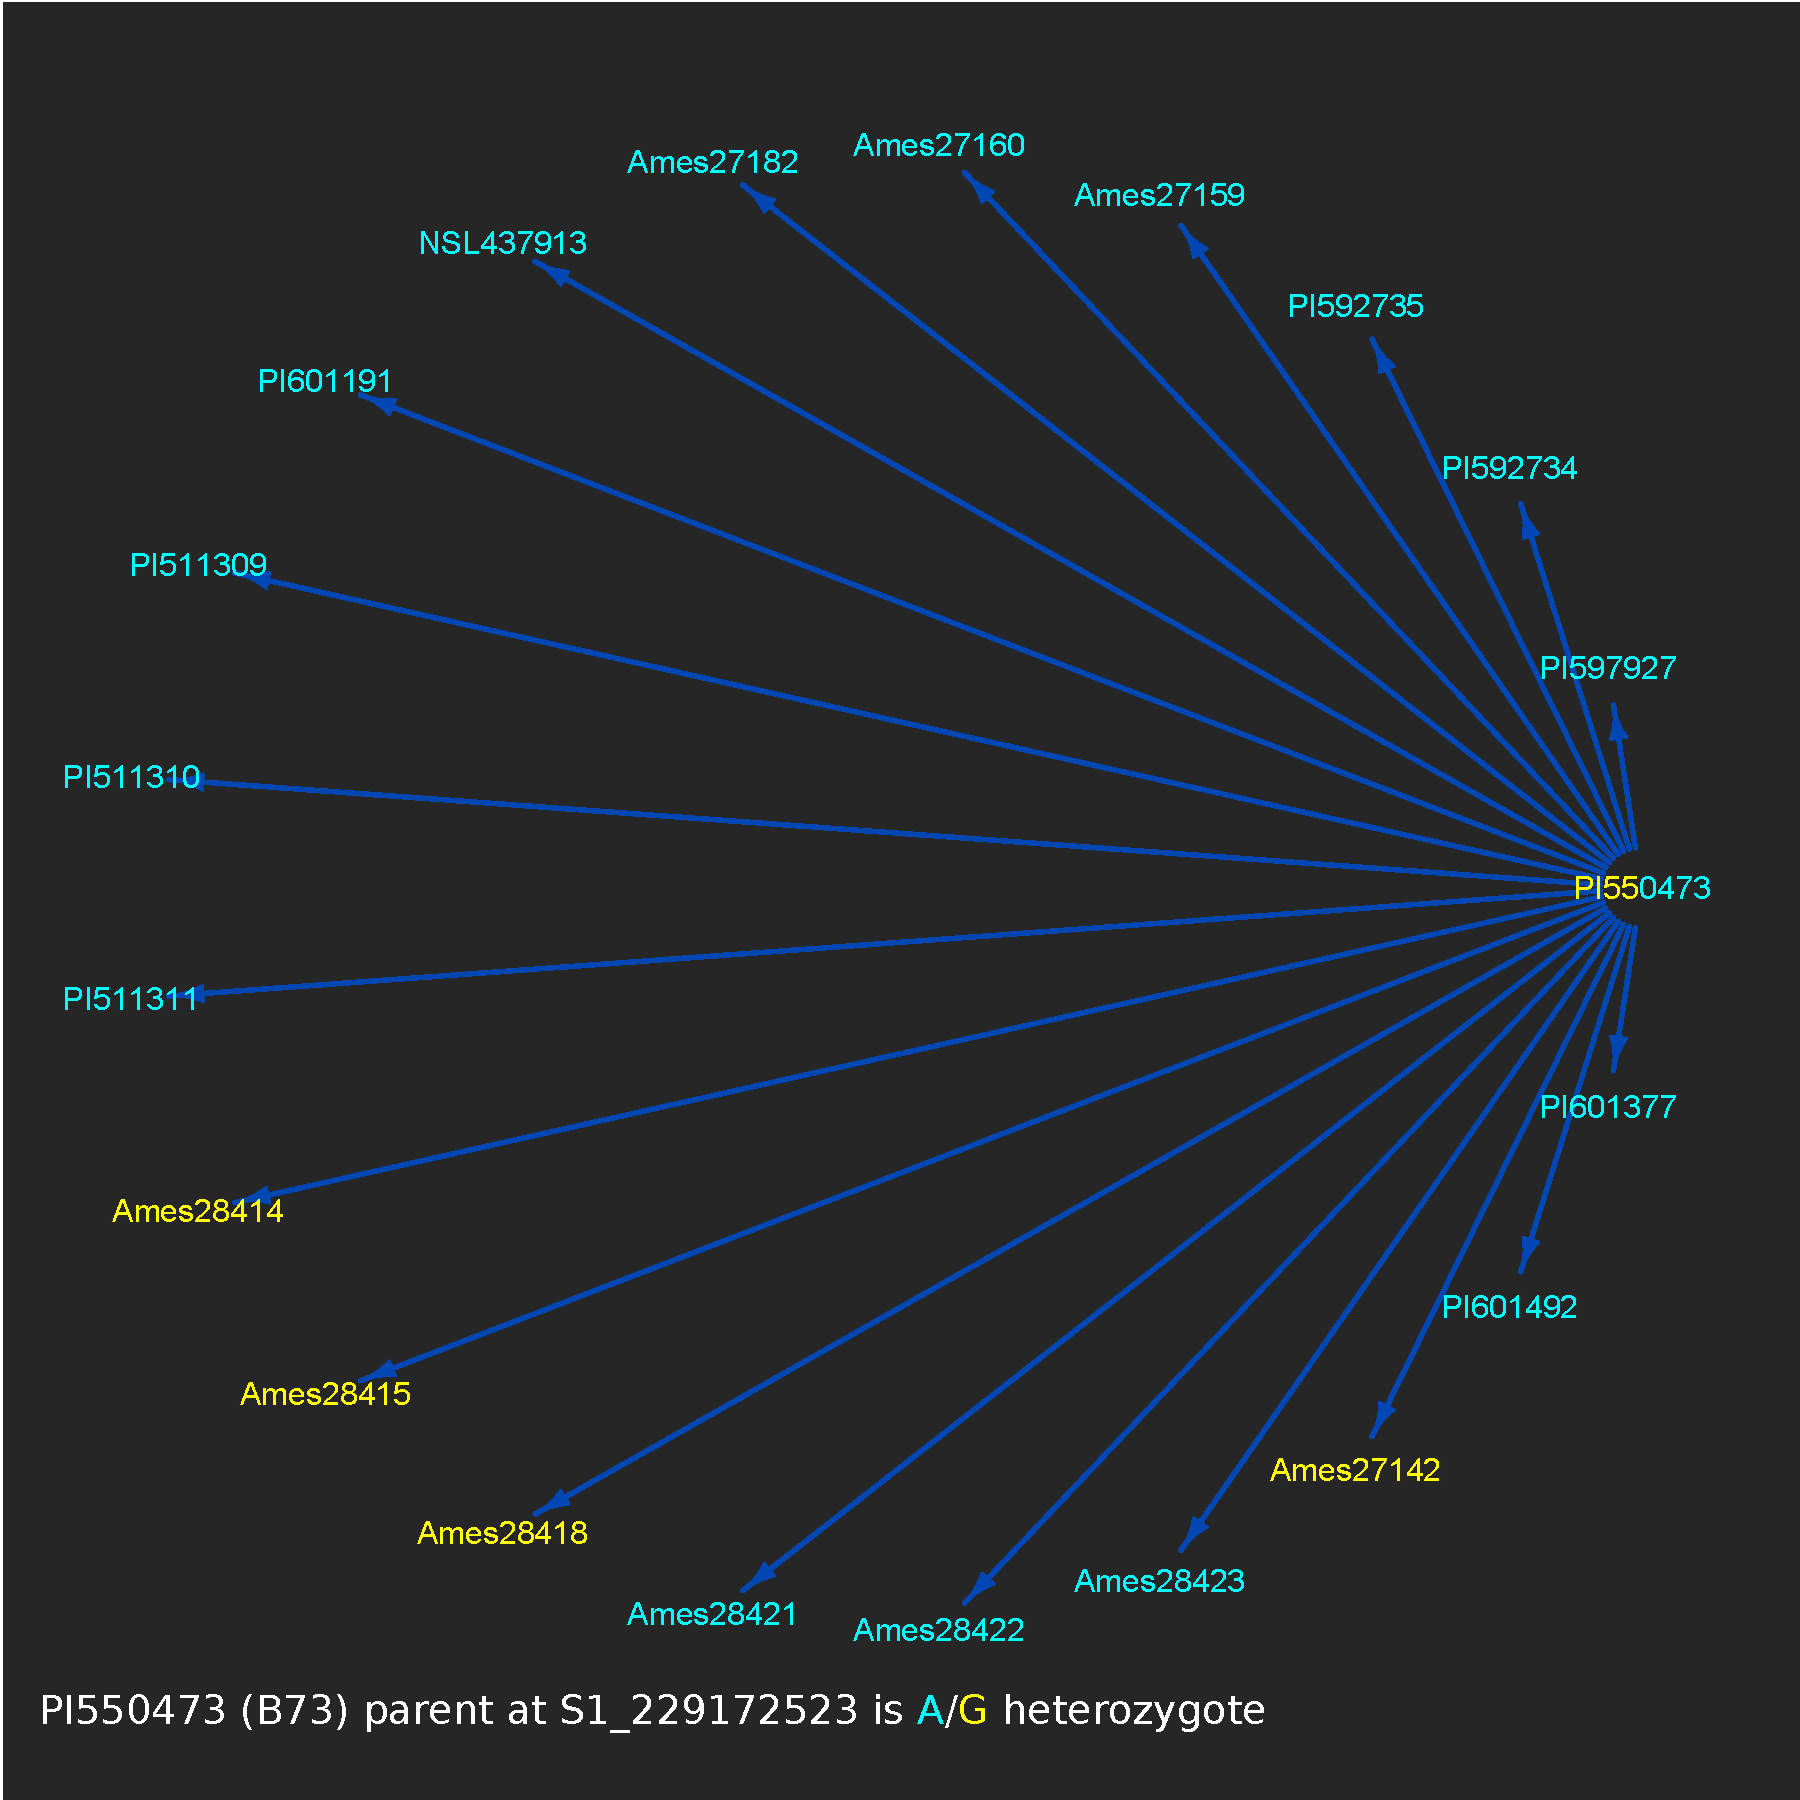
\includegraphics[width=1.0\linewidth]{Pruned.pdf}
\caption{B73 (also known as PI550473 by NPGS and a number of its inbred progeny) is heterozygous at 379 loci out of over 954000 loci with GBS markers). The blue labels represent which inbred progeny obtained the A allele, whereas the yellow labels indicate the progeny that have obtained the G allele at a particular locus. \textbf{NB: the other parent of these lines is not indicated for simplicity}.}
\label{fig:alleledrop}
\end{figure}






\subsubsection*{Project 2 for student 2: novel population genomics approaches to project current phenotypes back in time}
\label{}
Novel population genomic approaches described in \cite{Berg:2014bs} propose the idea of using a technique analogous to $Q_ST$ that it is possible to project current phenotypes (or phenotypes from one environment) back in time (to another environment)

\subsubsection*{Genotyping and grow out of lines that appear to feature heavily in the pedigree}
The inbreds that feature heavily in the historic pedigree will not only be genotyped, but phenotyped and grown out at the University of Delaware. This allow us to ground truth the expected results from using the approach in \cite{Berg:2014bs}


\subsection*{Expected outcomes \& Utility of results}

\subsubsection*{A user friendly, open database}

Our first expected deliverable is an open public pedigree database to be hosted on maize GDB for the long term future. Users will be able to contribute and revise incomplete information, with the goal of establishing a nearly complete public pedigree of maize inbred lines. \textbf{To our knowledge, this will be one of the first public crop databases of its kind (with lines having genomic and phenotypic data mapped onto entries).}
\par Ensuring data, code, and script are open-access or open-source (freely available to the public) is important for critique, debate, and dialogue in science. Dr. Ross-Ibarra has a long track record of ensuring openness with his science, data, and code. Throughout this project, both Dr. Ross-Ibarra and Dr. Crosby will endeavour to ensure that code and data are available via repositories such as github, figshare, maize GDB, and iPlant.

%\subsection*{The application of current cutting-edge population genomic approaches to quantitative genetics}

 

%\subsection*{}
%- Ground truth with actual grow-out
%- Way of discovering het error rates in GBS
%- identification of ghost ancestors?

\subsection*{Means of analysis/interpretation}
Dr. Randall Wisser has agreed to provide plot space for growing up germplasm of lines disproportionately present in the pedigree that have phenotypic data affiliated with their release sheets or with NPGS, i.e. drought resistance, heavy-metal tolerance, disease resistance, etc. The grow-out is to ground truth the suppositions gained from \citep{Berg:2014bs}.


\subsection*{Limitations \& Prospective pitfalls}
While we are very optimistic about the prospect of obtaining accurate pedigree information from these various institutions the nature of corn-breeding and record keeping of corn-breeding can be nebulous. Ideally, we would be able to accurately count the number of meioses in the total pedigree, in each heterotic group, down to each line; thus, retracing the complete ancestry of a given contemporary inbred. However, in many cases, it may not have been noted at which point in a breeding program a line was bulked at, nor on occasion which lines were used in recycling an inbred when seed was exhausted. For instance, a record from NPGS may indicate that a line was bulked and stored at cycle 6, or it may have been bulked and stored at cycle 4. As a ballpark figure, a ``cycle 6 inbred'' means that germplasm from that line is 99\% homozygous at all locus pairs. Meaning that if this inbred is selfed further, not much changes with respect to levels of homozygosity nor heterozygosity (as recombination via selfing is ineffective beyond this point).  Thus, so long as an inbred is at or beyond cycle 6, it will be kept, but inbreds before this period shall be discarded.

\par To ensure that historical records of inbred lines are isolated at cycle 6 and beyond we will investigate the level of heterozygosity in each of these lines with GBS data relative to the total amount of missing data in an individual line. Within a reasonable confidence limit most lines should show a very small portion of heterozygous loci even with GBS markers (known to have a high rate of error in undercalling heterozygous). 

\par Historical pedigree records and other information on old lines may be available, but the germplasm from these old lines may simply not be available (genomic data will not be able to be mapped onto these lines. Currently, we know that 12.9 In such cases, we would seek available germplasm from the next nearest relatives according to historical information. 


\subsection*{Hazards to personnel}
There will be car/air travel required by Dr. James Holland's masters student, CO-PI Dr. William Tracy, and the post-doc Dr. Kate Crosby) to the different land grant institutions. This travel is required for obtaining pedigree records from each land grant institution's library during year 1 of the proposed three year grant. Air travel will likely be necessary for the students and the post-doc to travel to a conference (most likely the Maize Genetics conference in 2016 or 2017) to present their results to the maize community at large. Travel is likely the most dangerous activity that any personnel will experience for the duration of this project, so we will take steps to ensure that all participants have travel insurance and benefits during these periods, and this is reflected in our current budget. 


\subsection*{Timeline}
A graphical timeline of our three-year proposal is presented below.
The first year will be spent traveling and gathering and digitizing pedigree records at land-grant institutions that have been identified by CO-PI Dr. William Tracy (one of two authors of the most authoritative public guide on the pedigrees of maize inbred lines to date) and senior personnel Dr. Oscar Smith (recently retired senior corn breeder who spent 30 + years with Dupont Pioneer) as having had breeding programs, but where records have not been digitized or made widely available. 
\par Dr. William Tracy and Dr. James Holland's masters student will largely be responsible for traveling to and scanning hard-copy records into digital format. Dr. William Tracy has committed to obtaining records from the University of Wisconsin, University of Nebraska, and will also visit the University of Florida. Dr. James Holland's student will be responsible for the breeding records at North Carolina State University, Virgina Tech, and the inbred records housed at the USDA at the University of Missouri. We estimate that this should take no longer than a few weeks at each institution with the first student or CO-PI. 
\par The scanned digital records must then be translated into a usable data format for further analysis with NGS or phenotype data. At worst, this will involve the student, CO-PI (Holland or Tracy) or the postdoc (Crosby), physically reading and translating each of the scanned papers, and this could take several months to the entire first year depending on volume of records. Dr. Kate Crosby with assistance from Dr. Oscar Smith, Dr. William Tracy, with cooperation from Dr. Taner Zen will be responsible for ensuring a consistent data format for hosting on maize GDB.
\par At the start of the second year, any inbred line that is disproportionately present in the pedigree with available germplasm, but that has no to little genetic information on it will be genotyped using the GBS platform. 
\par
Dr. Randall Wisser's student will then start and over a period of 3-6 months will learn the population genomics approach presented in \citep{Berg:2014bs}, as well as identify and incorporate phenotypic information into the database from the data gathered in year one. As a way of ground-truthing the phenotypic data and assessing the , Dr. Randall Wisser and his student will grow out lines used 




\bibliography{kc.bib,jri.bib}

\end{document}